\documentclass[tikz,border=10pt]{standalone}
\usepackage{tikz}
\usetikzlibrary{shapes.geometric, arrows.meta}

\tikzstyle{startstop} = [rectangle, rounded corners, minimum width=3cm, minimum height=1cm,text centered, draw=black, fill=red!30]
\tikzstyle{process} = [rectangle, minimum width=3cm, minimum height=1cm, text centered, draw=black, fill=orange!30]
\tikzstyle{decision} = [diamond, minimum width=3cm, minimum height=1cm, text centered, draw=black, fill=green!30]
\tikzstyle{arrow} = [thick,->,>=stealth]

\begin{document}
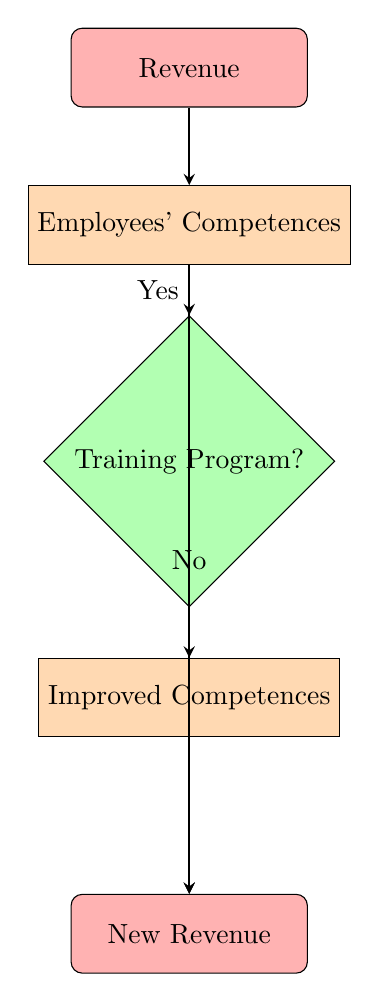
\begin{tikzpicture}[node distance=2cm]

    % Nodes
    \node (revenue) [startstop] {Revenue};
    \node (competences) [process, below of=revenue] {Employees' Competences};
    \node (training) [decision, below of=competences, yshift=-1cm] {Training Program?};
    \node (improved_competences) [process, below of=training, yshift=-1cm] {Improved Competences};
    \node (new_revenue) [startstop, below of=improved_competences, yshift=-1cm] {New Revenue};

    % Arrows
    \draw [arrow] (revenue) -- (competences);
    \draw [arrow] (competences) -- node[anchor=east] {Yes} (training);
    \draw [arrow] (competences) -- node[anchor=south] {No} (new_revenue);
    \draw [arrow] (training) -- (improved_competences);
    \draw [arrow] (improved_competences) -- (new_revenue);

\end{tikzpicture}
\end{document}